\documentclass[../main.tex]{subfiles}
\begin{document}
\chapter{Editor Features}
\label{chapter:editor-featres}

The Logical English editor provides various features that help the user understand, write, and correct Logical English.
\section{Highlighting}
\begin{figure}[h!]
\centering
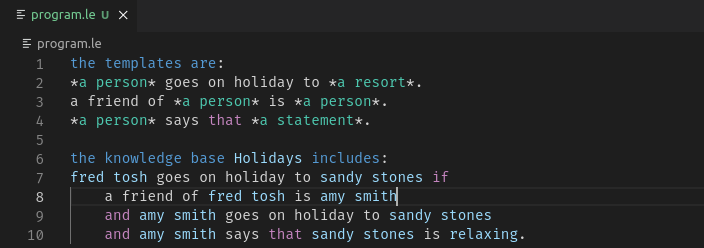
\includegraphics[width = \linewidth]{./figures/highlighting.png}
\caption{The editor highlighting grammatical components of a short Logical English program.}
\label{fig:highlighting}
\end{figure}
As shown in Figure \ref{fig:highlighting}, the editor highlights grammatical features of Logical English. These include the argument names of templates, logical connectives between atomic formulas, headers and their names, as well as the terms of atomic formulas. Figure \ref{fig:highlighting}, as well as subsequent screenshots, are taken with Visual Studio Code using the built-in `Solarized Dark' colour theme. Features of Logical English are highlighted regardless of the colour theme used, with the only change being the colours that features are given.

\section{Code Completion}\begin{figure}[h!]
\centering
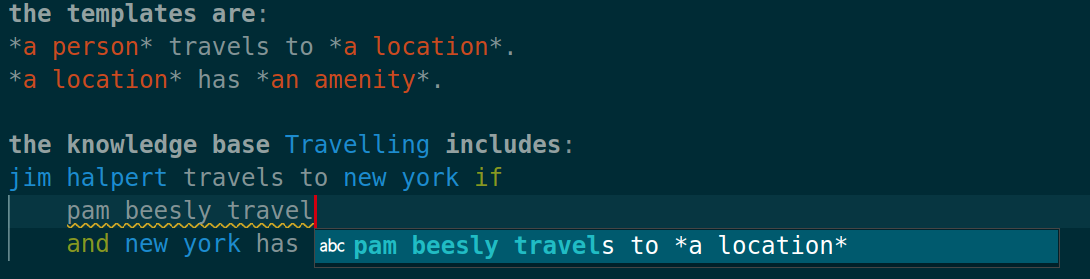
\includegraphics[width = \linewidth]{./figures/auto-suggest.png}
\caption{The editor suggesting the remainder of an incomplete atomic formula.}
\label{fig:code-completion}
\end{figure}
Figure \ref{fig:code-completion} shows the editor suggesting the remainder of an incomplete atomic formula. This happens as the user is typing the atomic formula, as soon as the atomic formula begins to conform to a template. When selecting the suggested formula, done by clicking on the suggestion or pressing Tab, the suggested atomic formula is inserted with the remaining arguments (such as `a location' in \ref{fig:code-completion}) being replaced by placeholders. The user can navigate across the placeholders by pressing Tab, allowing the user to fill in the placeholders efficiently.

\section{Error Diagnosis}
\subsection{Atomic formulas without templates}
\label{section:no-template-feature}
\begin{figure}[h!]
\centering
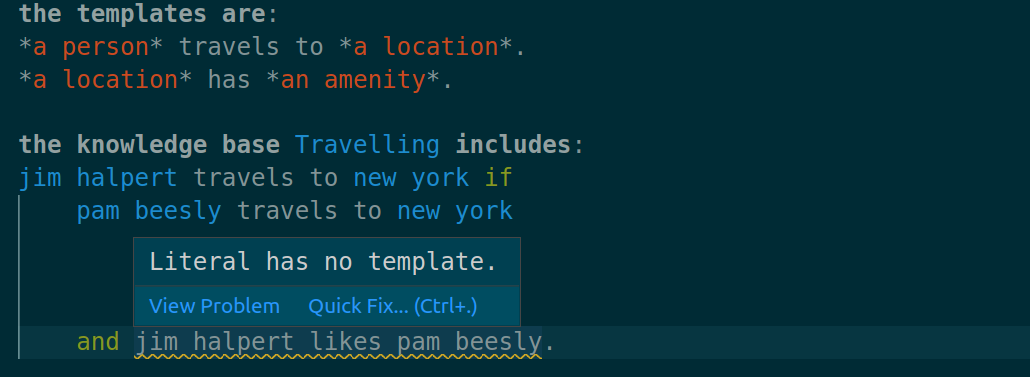
\includegraphics[width = \linewidth]{./figures/literal-wo-template.png}
\caption{The editor identifying an atomic formula that does not match any of the templates.}
\label{fig:no-template-diag}
\end{figure}
If the document contains an atomic formula that does not conform to any template, the editor marks the atomic formula with an underline representing a `warning'. On hovering over the atomic formula, the editor produces an explanatory error message. This is shown in figure \ref{fig:no-template-diag}.
\\ 
\\
This feature occurs when an atomic formula does not conform to any template written in the document, nor any of Logical English's pre-defined templates.

\section{Clauses with misaligned connectives}
\begin{figure}[h!]
\centering
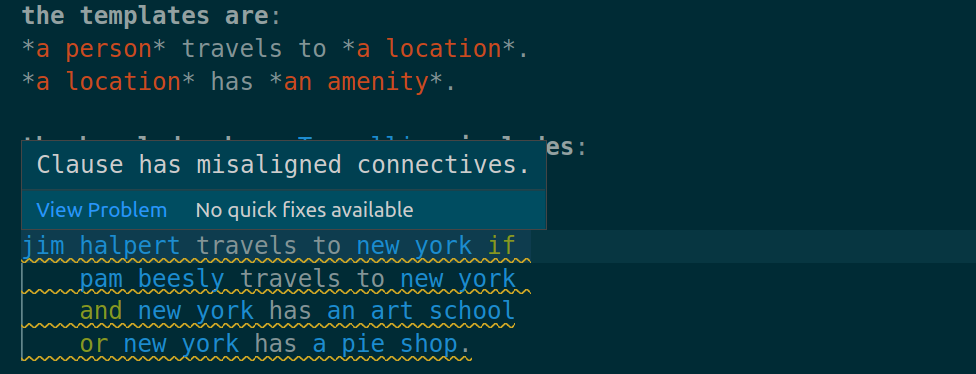
\includegraphics[width = \linewidth]{./figures/misaligned-connectives.png}
\caption{The editor identifying a clause with misaligned connectives.}
\label{fig:misaligned-connectives}
\end{figure}
If the document contains a clause which has connectives whose order of precedence is not stated through indentation (as discussed in section \ref{section:knowledge-base}), the editor marks the clause with an underline representing a `warning'. On hovering over the clause, the editor produces the error message `Clause has misaligned connectives.'. This is shown in figure \ref{fig:misaligned-connectives}.

\section{Code Actions}
\begin{figure}[h!]
\centering
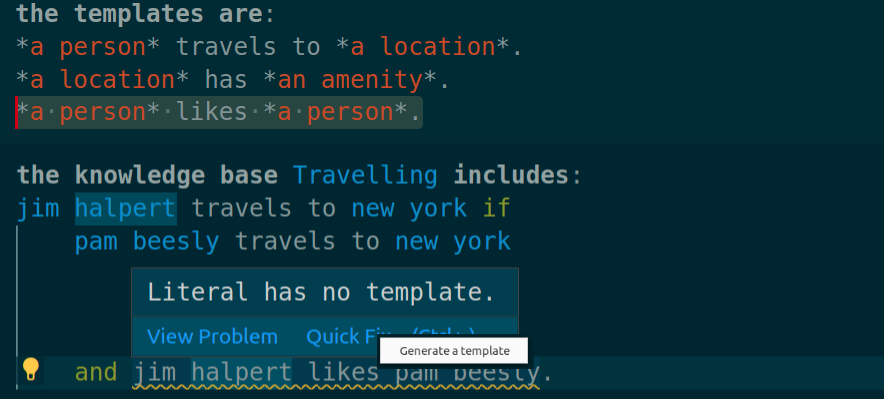
\includegraphics[width = \linewidth]{./figures/generate-template-full.png}
\caption{The editor generating a new template to match template-less atomic formulas.}
\label{fig:new-template}
\end{figure}
Figure \ref{fig:new-template} shows the process of generating a new template that conforms to atomic formulas. If a number of atomic formulas are marked as not conforming to any templates (discussed in section \ref{section:no-template-feature}), hovering over any one of the atomic formulas and selecting `Quick Fix' produces the `Generate a template' option. When pressed, the editor generates a single template that conforms to every atomic formula that was marked with this error. 
\\
\\
If the marked atomic formulas contain terms which also feature in unmarked atomic formulas, then the types of those terms will feature in the template. This is shown in Figure \ref{fig:new-template}: the terms \codeword{jim halpert} and \codeword{pam beesly} feature in unmarked atomic formulas and have type \codeword{a person}. This allows the generated template to feature the type \codeword{a person}.

\section{Type Checking}
\subsection{Type Mismatch Errors}
\begin{figure}[h!]
\centering
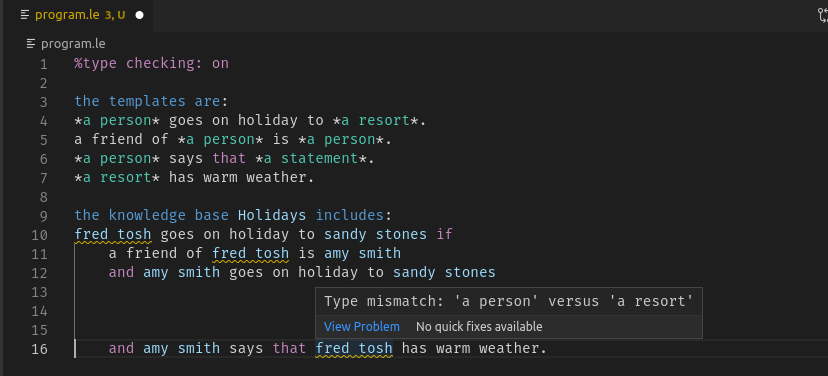
\includegraphics[width = \linewidth]{./figures/type-error.png}
\caption{The editor identifying a type mismatch scenario. The term \codeword{an art school} appears across two atomic formulas. The term is assigned the type \codeword{a location} in the first atomic formula, but is assigned the type \codeword{an amenity} in the second. These types do not have the same name, nor is one a sub-type of the other.}
\label{fig:type-mismatch}
\end{figure}
The comment %\codeword{%type checking: on}
(shown at the top of Figure \ref{fig:type-mismatch}) activates type checking features in the editor. If the following scenario occurs:
\begin{enumerate}
    \item an atomic formula contains a term $x$, where $x$ is assigned the type $A$
    \item another atomic formula in the same clause contains the same term $x$, but $x$ is assigned the type $B$
    \item $A$ and $B$ do not have the same name, nor is one a sub-type of the other (discussed further in section \ref{section:type-hierarcy-features}).
\end{enumerate}
then all the instances of the term are marked as warnings. If any one of the terms are hovered over, a message appears that explains that there is a type mismatch between the two stated types.

\subsection{The Type Hierarchy}
\label{section:type-hierarcy-features}
\begin{figure}[h!]
\centering
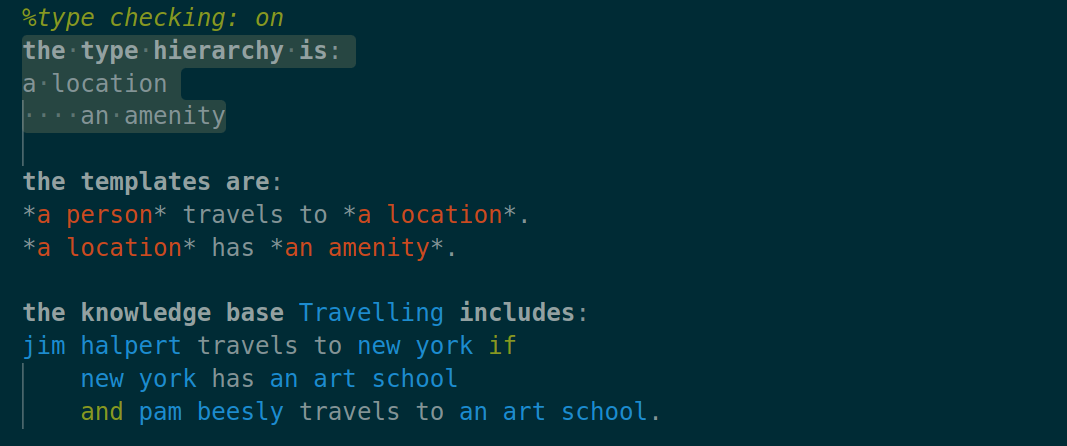
\includegraphics[width = \linewidth]{./figures/type-hierarchy.png}
\caption{A type hierarchy that resolves the type mismatch error in Figure \ref{fig:type-mismatch}. The type \lstinline{a location} is now a subtype of \codeword{an amenity}.}
\label{fig:type-hierarchy}
\end{figure}
The header \codeword{the type hierarchy is:} marks the optional `type hierarchy' section where a type hierarcy can be written. To write that the type $B$ is a subtype of the type $A$, write the type name of $B$ on a line below the type name of $A$, indented further than $A$'s type name by a single tab. Continue this way with multiple types to form an indented list of the types.
\\
The editor will use this type hierarchy in checking for type errors. For instance, in Figure \ref{fig:type-hierarchy}, the type hierarchy states that type \codeword{an amenity} is a subtype of the type\codeword{a location}. This means that the usage of the term \codeword{art school} in the knowledge base does not result in a type mismatch error. Although the term is assigned two types, one type is now the subtype of the other.
\end{document}